\documentclass{article}

\usepackage[utf8]{inputenc}
\usepackage[T1]{fontenc}
\usepackage{geometry}
\usepackage{graphicx}   %ALLOWS INSERTING IMAGES (AND MAYBE SOME MORE STUFF) %
\usepackage{subcaption} %ALLOWS CAPTIONS FOR SUBFIGURES%
\usepackage{verbatim} % ALLOWS MULTILINE COMMENTS WITH \begin{comment} AND \end{comment} %
\usepackage{amsmath,amssymb} % PERMETTE L'USO DI SIMBOLI MATEMATICI "AVANZATI" COME 'MINORE O UGUALE' E ALTRI %
\usepackage{amstext}

\geometry{a4paper}
                        %Una riga vuota tra due scritte spazia di una riga anche sul pdf. Andare a capo una volta non provoca nulla nel pdf%
\usepackage[italian]{babel}
%\usepackage[french, italian]{babel} non funzione per motivi a me ignoti
\frenchspacing %cos'è?

%%%  INTESTAZIONE  %%%

\title{Relazione dell'esperimento di misura della velocità della luce}
\author{Lorenzo Ramella, Alessandro Matteo Rossi, Marco Tambini}
\date{\today}


%%%  INIZIO DOCUMENTO  %%%

\begin{document}
\maketitle

%%%  ABSTRACT  %%%

\begin{abstract}
L’esperimento si propone di misurare la velocità delle luce usando il metodo di Focault. %%da modificare
\end{abstract}

%%%  INDICE  %%%%

\tableofcontents

\section{Introduzione teorica}
Il metodo di Focault per la misura della velocità della luce consiste nell'uso di uno specchio rotante, che riflette la luce emessa da una sorgente su di uno specchio concavo. 

Una sorgente luminosa $S$ emette una luce che, opportunamente diaframmata da una lente $L_1$, attraversa una lastra semitrasparente angolata di 45° rispetto alla direzione del fascio. Una lente $L_2$ focalizza il fascio nel punto $S'$ sullo specchio concavo, dopo essere stata deflessa dallo specchio rotante. La luce riflessa dallo specchio concavo viene deflessa nuovamente dallo specchio rotante, che nel frattempo ha ruotato di un angolo 

\[\alpha = \omega \frac{2D}{c}\]

dove $\omega$ è la velocità angolare dello specchio e $D$ è la distanza tra lo specchio rotante e lo specchio concavo.

Il fascio luminoso di ritorno sulla lente $L_2$ viene focalizzato come se provenisse da una sorgente $S''$ spostata da $S'$ di una quantità 

\[\Delta = 2 \alpha D\] 

Tenendo presente che il fattore di amplificazione $G$ della lente $L_2$ è esprimibile mediante la seguente relazione:

\[G=\frac{b}{D+a}\]

dove $b$ è la distanza tra $L_2$ e la sorgente luminosa e $a$  la distanza tra $L_2$ e lo specchio rotante. Lo spostamento laterale $\delta$ dell'immagine è quindi:

\[\delta = G\Delta =\frac{2\alpha b D}{D + a}=\frac{4 D^2 b \omega}{c(D+a)}\]

È possibile ricavare $b$ dalla legge dei punti coniugati. Sapendo che:

\[\frac{1}{b}+\frac{1}{D+a}=\frac{1}{f_2}\]

Si deduce che:

\[b=\frac{f_2(D+a)}{D+a-f_2}\]

E quindi, conoscendo l'espressione di $\delta$ in cui compare $c$ e avendo ricavato l'unica variabile incognita $b$, si ottiene:

\[c= \frac{4f_2D^2(\omega-\omega_0)}{[(D+a+f_2)\Delta\delta]}\]

dove $\omega_0$ è la velocità angolare iniziale e $\Delta\delta = \omega - \omega_0$ è lo spostamento dell'immagine della sorgente luminosa.


% \begin{comment}
\begin{figure}[h]
    \centering
        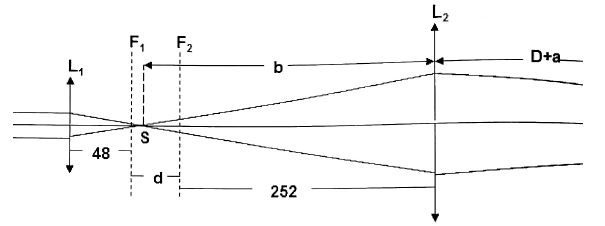
\includegraphics[width=\linewidth]{IntroTeorica1.JPG}
    \caption{Schema apparato - intorno del beam-splitter}
\end{figure}
% \end{comment}

\section{Progettazione dell'esperimento}
Il banco ottico di laboratorio era composto da una sorgente luminosa e un sistema di lenti e specchi, il tutto ancorato saldamente alle varie parti del banco mediante morse.

\begin{figure}[h] %here, top, bottom, ! = forza posizionamento dove latex riesce, H mettilo dove cazzo dico io%
    \centering
    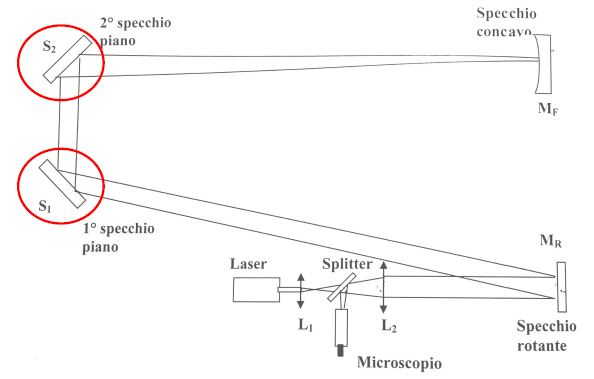
\includegraphics[width=0.6\linewidth]{Progettazione1.JPG}
    \caption{Schema dell'apparato di laboratorio}
    \label{schema_apparato}
\end{figure}

Prima di cominciare le misure di $c$ è necessario assicurarsi che gli elementi del banco ottico siano correttamente posizionati.

\vspace{1mm}

In principio abbiamo misurato la lunghezza del percorso compiuto dal raggio luminoso dallo specchio rotante allo specchio concavo. Per fare ciò abbiamo raccolto 4 misure
per le distanze %%%%%%%%%%%%%%
Come mostrato in Figura \ref{schema_apparato}, la sorgente luminosa coerente è un laser A CHE COSA?? fissato magneticamente a un binario graduato. La luce incontra una 
prima lente $L_1$ posta a distanza ??????. 
Siccome la luce incidente sulla lente proviene "dall'infinito" (le dimensioni lineari della lente sono molto ridotte rispetto alla distanza tra laser e $L_2$) essa viene
rifratta nel suo fuoco, che il produttore della lente dichiara essere a una distanza $f_1 = INSERIRE$. A distanza $f_1$ da $L_1$ è posto il beam-splitter, un elemento
dotato di uno specchio semiriflettente orientato a 45° rispetto alla luce incidente, che permette di trasmettere la luce in arrivo alla lente $L_2$. La lente $L_2$ 
è posta a distanza $b = ???$ dal beam-splitter e trasmette a sua volta la luce allo specchio rotante. Per permette alla luce di percorrere il sistema di specchi specchio
rotante - $S'$ - $S''$ - specchio concavo bisogna agire sulla cinghia dello specchio rotante per riflettere il raggio incidente approssimativamente al centro di $S'$.
Fatto questo si regola l'inclinazione di $S'$ per riflettere il raggio proveniente dallo specchio rotante approssimativamente nel centro di $S''$, attraverso due
viti micrometriche poste dietro lo specchio. Si ripete quest'ultimo procedimento per potare il raggio dal centro di $S''$ al centro dello specchio concavo.

\vspace{1mm}

Raggiunta la condizione di raggio che percorre tutta la lunghezza $D$, è necessario agire nuovamente sulle viti micrometriche degli specchi per fare tornare il raggio
luminoso indietro fino al beam-splitter ripercorrendo il suo cammino di andata.
% DA RIVEDERE


Problemi tecnici riscontrati: 

\section{Misure}

\section{Analisi dei dati}

\section{Conclusioni}

\section{Appendice}

\end{document}


% Å ^{\circ} \vspace{1mm} per spaziare verticalmente \begin{equation} e \end{equation} con dentro un \label e fuori un \ref per numerare e avere il riferimento alle
% equazioni


